\chapter{Appendix}

\section{Additional channel networks}
\label{appendix_networks}

\subsection{Second interval mainnet}

\begin{figure}[ht]
    \centering
    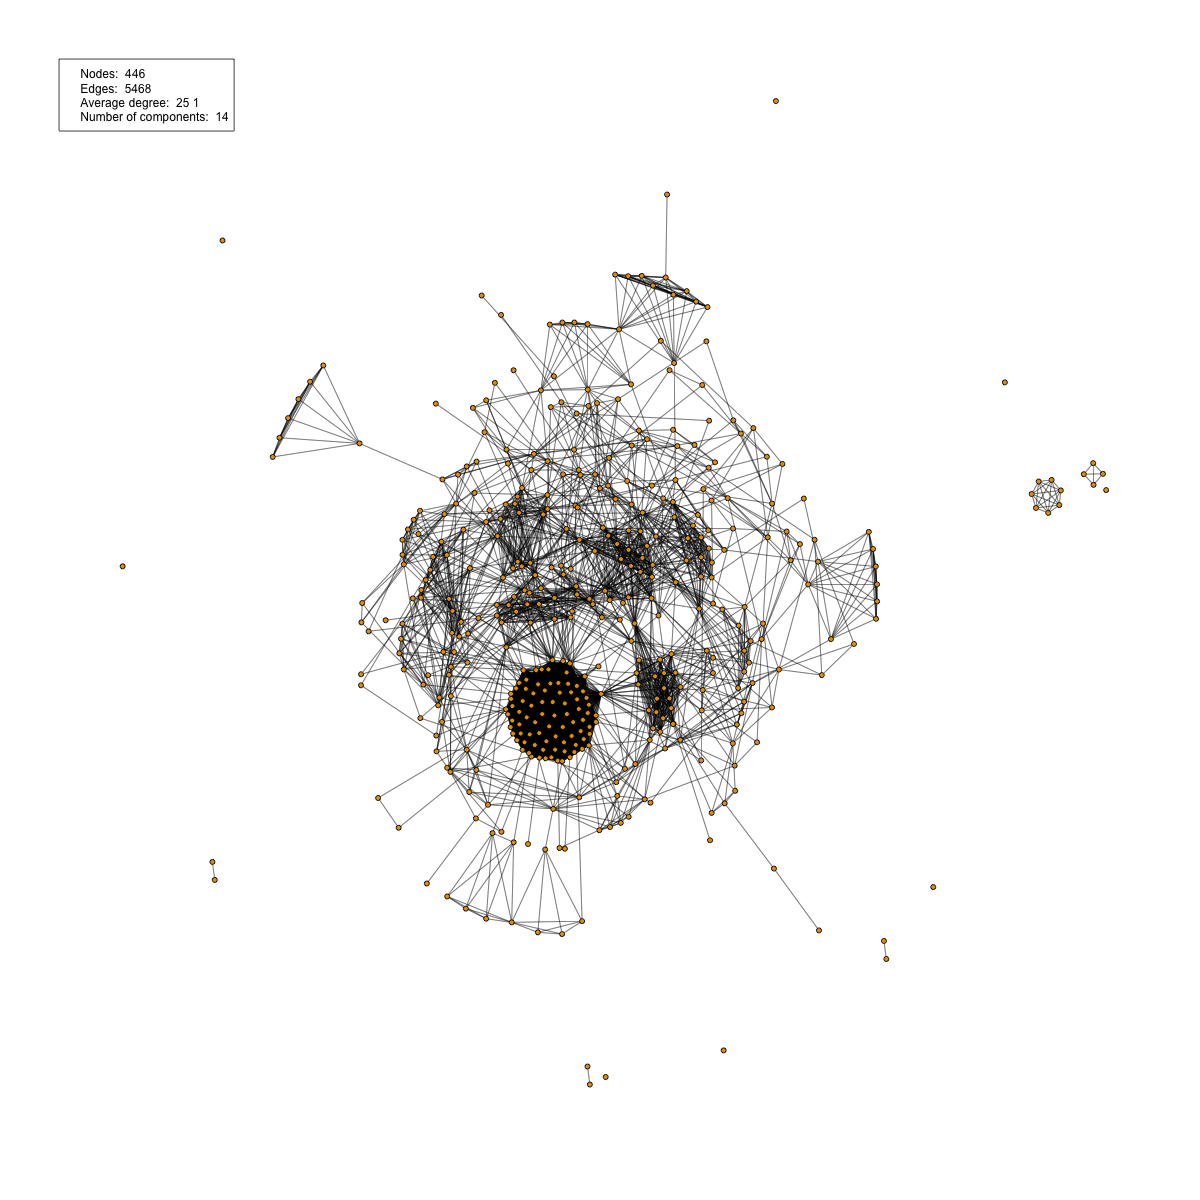
\includegraphics[width=14cm]{figures/graphs/cg_ln_mainnet_run2.png}
    \caption{Linked channels from the LN, mainnet, second interval}
    \label{fig:channel_network_LN_mainent2}
\end{figure}

\begin{figure}[H]
    \centering
    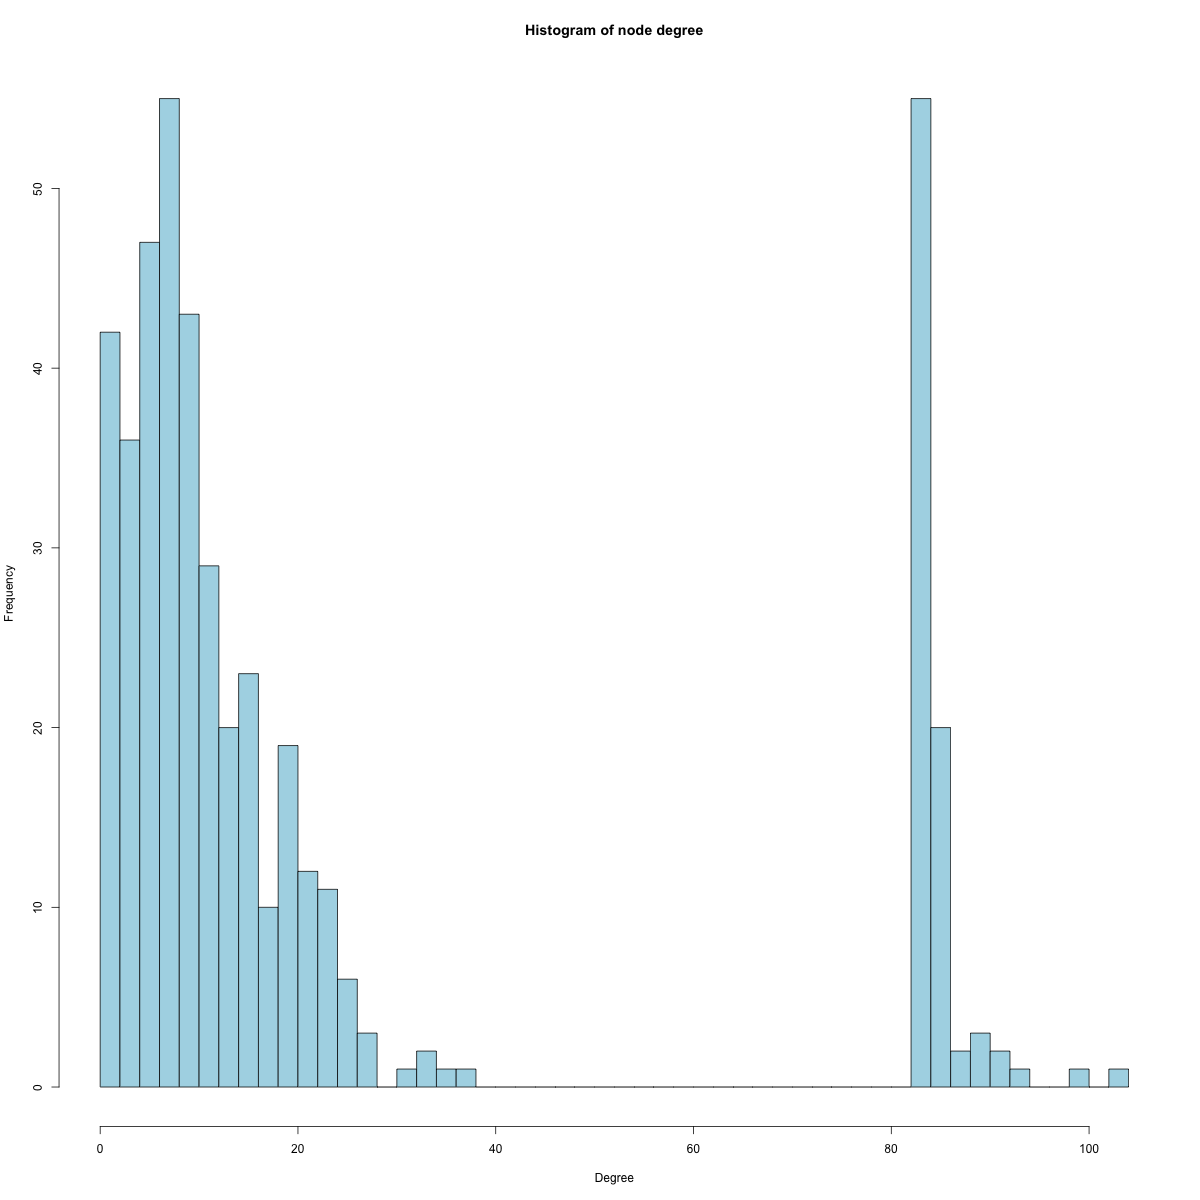
\includegraphics[width=16cm]{figures/graphs/histogram_ln_mainnet_run2.png}
    \caption{Histogram of node degree for the network in \cref{fig:channel_network_LN_mainent2}}
    \label{fig:histogram}
\end{figure}

\begin{figure}[H]
    \centering
    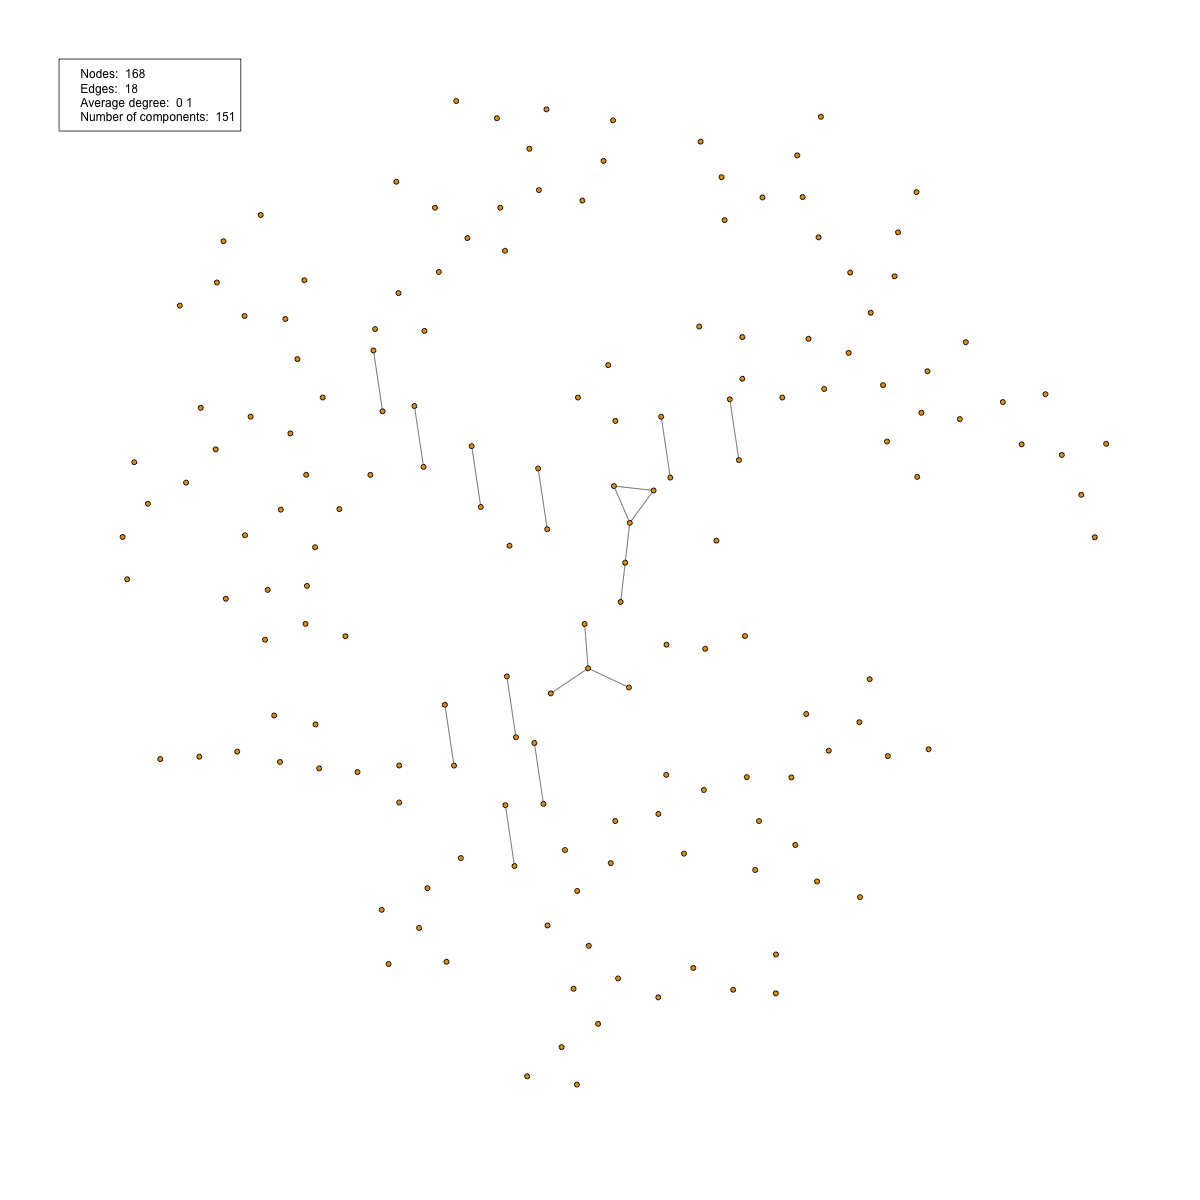
\includegraphics[width=14cm]{figures/graphs/cg_bc_mainnet_run2.png}
    \caption{Linked channels from the blockchain, mainnet, second interval}
    \label{fig:channel_network_BC_mainnet}
\end{figure}


\subsection{Testnet}

\begin{figure}[ht]
    \centering
    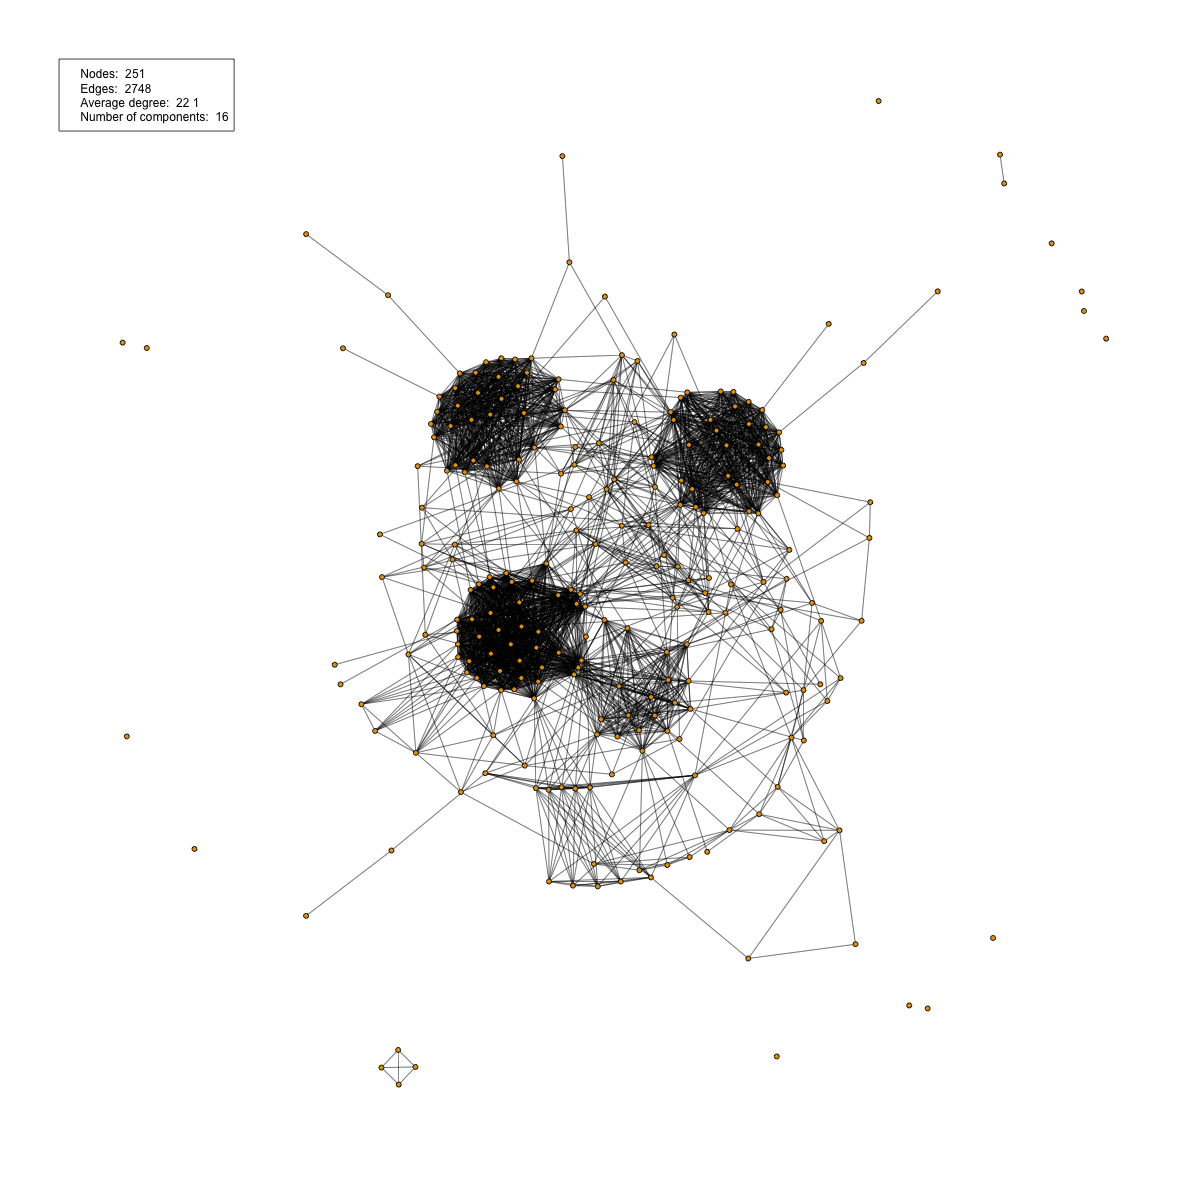
\includegraphics[width=14cm]{figures/graphs/cg_ln_testnet_run1.png}
    \caption{Linked channels from the LN testnet, from interval one}
    \label{fig:channel_network_LN_testnet}
\end{figure}

\begin{figure}[H]
    \centering
    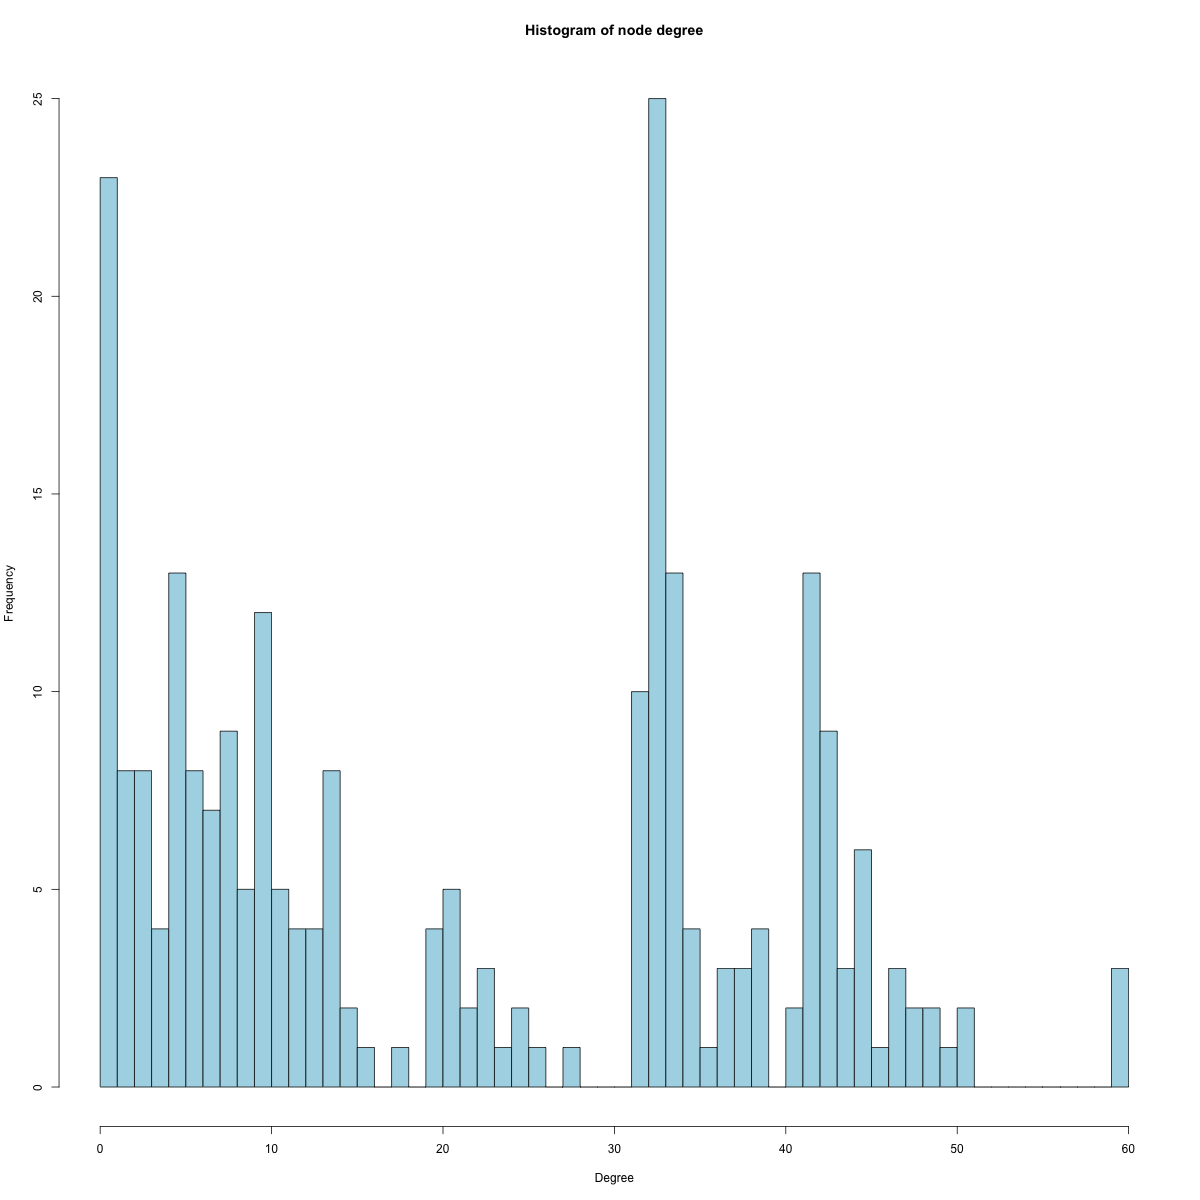
\includegraphics[width=16cm]{figures/graphs/histogram_ln_testnet_run1.png}
    \caption{Histogram of node degree for the network in \cref{fig:channel_network_LN_testnet}}
    \label{fig:histogram}
\end{figure}

\begin{figure}[H]
    \centering
    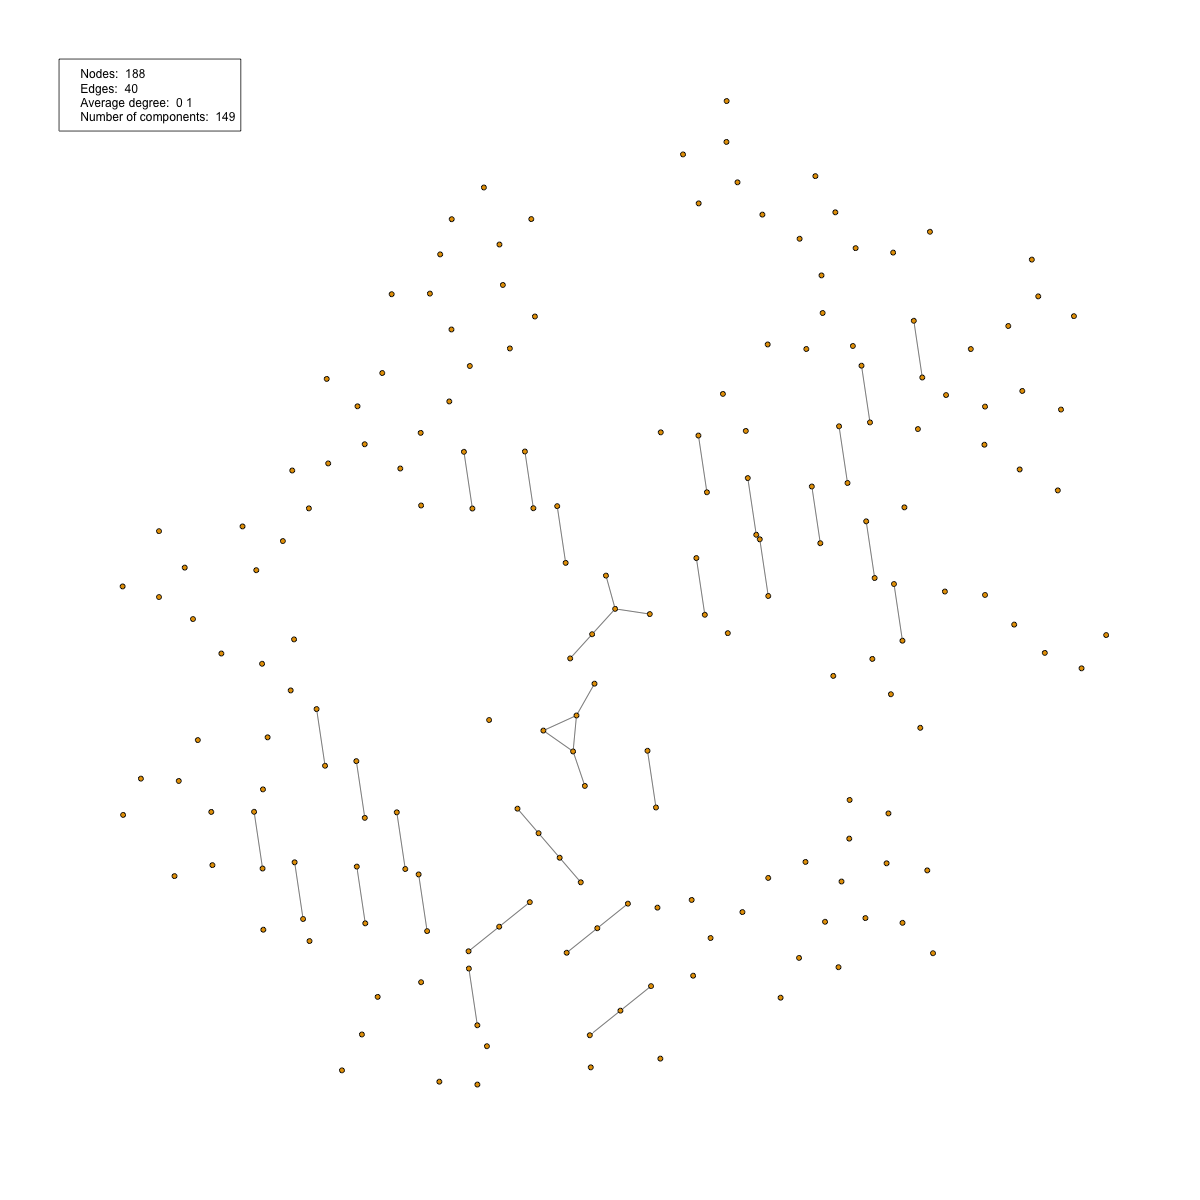
\includegraphics[width=14cm]{figures/graphs/cg_bc_testnet_run1.png}
    \caption{Linked channels from the testnet blockchain, from interval one}
    \label{fig:channel_network_BC_testnet}
\end{figure}
